\chapter{Planificación} 

\section{Temporización}

El proyecto ha tenido una investigación previa entre los meses de enero y marzo y ha sido planteado para su desarrollo entre mitad de marzo y principio de julio de 2022. El tiempo de desarrollo se ha dividido en sprints con una duración orientativa de 2 semanas. El significado de esto se desarrollará junto con el resto de la metodología en la siguiente sección. En la figura \ref{fig:roadmap} sobre la hoja de ruta del proyecto en su últimas etapas se puede consultar la distribución de los diferentes sprints en el tiempo.

\section{Metodología utilizada}

La metodología de diseño y desarrollo llevada a cabo está inspirada fuertemente por SCRUM, con algunas modificaciones dadas las condiciones del proyecto. Además, se ha llevado acabo un proceso de TDD. Las condiciones del proyecto que han condicionado la propuesta de proyecto son las siguientes:

\begin{itemize}
    \item \textbf{El perfil de usuario final.} El software a desarrollar no es un producto de usuario en el sentido tradicional. Es una serie de herramientas de desarrollo que serán utilizadas por otros programadores. Así, los usuarios son los desarrolladores que usarán el software.

    \item \textbf{La complejidad del MVP.} El modelo de datos y cómputo de GenoMus está altamente entrelazado. Esto aumenta la complejidad de la creación de cortes verticales\footnote{Más información sobre la verticalidad y horizontalidad de un subconjunto funcional en el siguiente artículo divulgativo: \url{http://www.deltamatrix.com/horizontal-and-vertical-user-stories-slicing-the-cake/}} de grupos funcionales que podrían corresponder a hitos.
    
    \item \textbf{La inestabilidad de la capacidad del equipo de desarrollo.} El equipo de desarrollo no se podía alejar más de lo defendido como ideal por SCRUM\footnote{En la sección 4.5 de la descripción original de la metodología SCRUM\cite{scrum} podemos encontrar la siguiente frase que resume las características principales del equipo de desarrollo: \textit{"The team that works on the new release includes full time developers and external parties who will be affected by the new release, such as marketing, sales, and customers"}. Debido a las características del proyecto, solo se cuenta con un desarrollador: el autor, y con un stakeholder: José López Montes, ambos trabajando lejos de a tiempo completo en este fork del proyecto GenoMus}. La baja capacidad de desarrollo y la variablidad de esta implica un aumento del riesgo de no llegar a las fechas de entrega.
\end{itemize}

Ante estas condiciones, se ha llevado a cabo un proceso de desarrollo con las siguientes características:

\begin{itemize}
    \item \textbf{División de las funcionalidades en historias e hitos.} Las funcionalidades técnicas del producto se han dividido según el método usual en metodologías ágiles. 
    
    \item \textbf{División temporal del trabajo en sprints.} El tiempo de desarrollo se ha dividido en sprints como es usual. Los sprints del proyecto han contado con la peculiaridad de ser de tiempo variable debido a la capacidad variable de desarrollo. Los sprints han durado el tiempo necesario para completar los objetivos asignados. Finalmente, los sprints han durado una media de tres semanas.

    \item \textbf{Testeo a través de tests automáticos}. Los flujos de usuario del prototipo trabajan con las estructuras de más alto nivel de GenoMus. Al ser estas estructuras dependientes del modelo de cómputo subyacente, se ha propuesto este modelo de cómputo junto con alguna funcionalidad básica como MVP. Al no respaldar ningún flujo de usuario, el desarrollo del MVP se ha realizado utilizando TDD como verificación de correctitud.
    
    \item \textbf{Planificación dinámica de historias e hitos.} El proyecto cuenta con varios ámbitos de incertidumbre los cuales han imposibilizado el análisis de requisitos funcionales completo previo al comienzo del desarrollo. Incluso la viabilidad del producto en el tiempo propuesto era desconocida. Así, el análisis completo de requisitos se ha llevado a cabo durante el desarrollo del MVP.
\end{itemize}

\subsection{Relación con SCRUM}

Como ya se ha mencionado, la metodología utilizada está fuertemente influenciada por SCRUM. Las diferencias con una implementación pura de la metodología recaen sobre las características atípicas del proceso de desarrollo mencionadas previamente. A continuación se realiza una exposición de la metodología de desarrollo realizada a través de una comparación con los procedimientos definidos en el artículo original de SCRUM\cite{scrum}. Esto queda expuesto en las siguientes tablas clasificadas por etapa del desarrollo: etapa de planificación en la tabla \ref{tab:met_planificacion}, etapa de diseño en la tabla \ref{tab:met_diseño}, etapa de desarrollo en la tabla \ref{tab:met_desarrollo} y etapa de clausura en la tabla de \ref{tab:met_clausura}.

\renewcommand{\arraystretch}{1.5}

\begin{table}[]
    \centering
    \begin{tabular}{p{5cm} p{6cm}}
        \multicolumn{2}{c}{\textbf{Comparación con SCRUM en etapa de planificación}} \\
        \hline 
        \textbf{Definición original} & \textbf{Implementación en este proyecto} \\ \hline \hline
        
        \textit{Development of a comprehensive backlog list.} & Se declara un \textit{backlog} extensivo previo al comienzo del primer sprint. Esta primera iteración del backlog contiene historias e hitos suficientes para desarrollar la primera iteración del software. \\ \hline
        
        \textit{Definition of the delivery date and functionality of one or more releases.} & Se define la fecha de entrega del proyecto como el 8 de julio de 2022. \\ \hline
        
        \textit{Selection of the release most appropriate for immediate development.} & Se define un MVP de cara a la primera \textit{release}. \\ \hline
        
        \textit{Mapping of product packets (objects) for backlog items in the selected release} & Se define una correspondencia de hitos a completar en cada \textit{release}. \\ \hline
        
        \textit{Definition of project team(s) for the building of the new release.} & El equipo de desarrollo está definido en todo momento y consiste únicamente en el autor de esta memoria. \\ \hline
        
        \textit{Assessment of risk and appropriate risk controls.} & Se reconoce el riesgo del MVP planeado y se mitiga con la propuesta de sprints flexibles. \\ \hline
        
        \textit{Review and possible adjustment of backlog items and packets.} & Se revisa la completitud y correctitud del backlog de manera previa a la definición de cada iteración del software. \\ \hline
        
        \textit{Validation or reselection of development tools and infrastructure} & Se validan las herramientas e infraestructura de desarrollo. Esto se hace en una prueba de concepto previa al inicio del primer sprint, como parte del proceso de análisis. \\ \hline
        
        \textit{Estimation of release cost, including development, collateral material, marketing, training, and rollout.} & Se estiman los costes de publicación de una iteración del software como el coste de diseño y el coste de desarrollo. Estas estimaciones quedan reflejadas como punto de historia asociadas a las historias de usuario individuales. \\ \hline
        
        \textit{Verification of management approval and funding.} & Este punto queda fuera de la planificación del proyecto por las condiciones de desarrollo. \\ 
    \end{tabular}   
    \caption{Comparación de SCRUM con la metodología realizada. Etapa de planificación.}
    \label{tab:met_planificacion}
\end{table}

\begin{table}[]
    \centering
    \begin{tabular}{p{5cm} p{6cm}}
        \multicolumn{2}{c}{\textbf{Comparación con SCRUM en etapa de diseño}} \\
        \hline 
        \textbf{Definición original} & \textbf{Implementación en este proyecto} \\ \hline \hline
        
        \textit{Review assigned backlog items.} & Tras la asignación de una historia de usuario en el sprint, se procede a realizar una revisión de la correctitud de las especificaciones técnicas de esta, alterándolas si es necesario. \\ \hline
        
        \textit{Identify changes necessary to implement backlog items.} & Una vez revisadas las especificaciones técnicas se realiza un diseño del código previo al desarrollo. Para esto se han utilizado herramientas como esquemas o pseudo-código. \\ \hline
        
        \textit{Perform domain analysis to the extent required to build, enhance, or update the domain models to reflect the new system context and requirements.} & Se ha realizado siempre un diseño orientado a iteraciones, evitando en la medida de lo posible el solapamiento de secciones afectadas por distintas funcionalidades. \\ \hline
        
        \textit{Refine the system architecture to support the new context and requirements.} & El propio diseño de los tipos de datos básicos o de la arquitectura del código ha sido modificado de manera iterativa para ajustarse a los requerimientos del desarrollo. \\ \hline
        
        \textit{Design review meeting, each team presenting approach and changes to implement each backlog item. Reassign changes as required.} & No aplica dadas las condiciones de desarrollo. \\ 
    \end{tabular}                   
    \caption{Comparación de SCRUM con la metodología realizada. Etapa de diseño de arquitectura o a alto nivel.}
    \label{tab:met_diseño}
\end{table}

\begin{table}[]
    \centering
    \begin{tabular}{p{5cm} p{6cm}}
        \multicolumn{2}{c}{\textbf{Comparación con SCRUM en etapa de desarrollo}} \\
        \hline 
        \textbf{Definición original} & \textbf{Implementación en este proyecto} \\ \hline \hline
        
        \textit{Meeting with teams to review release plans} & No aplica debido a las condiciones de desarrollo. \\ \hline
        
        \textit{Distribution, review and adjustment of the standards with which the product will conform.} & Al comienzo del sprint se declara el objetivo de éste. \\ \hline
        
        \textit{Iterative Sprints, until the product is deemed ready for distribution.} & En cada fin de sprint, el software cuenta con un subconjunto de las funcionalidades listas para su uso. Es desplegable y usable por un usuario. \\ \hline
        
        \textit{Develop: Defining changes needed for the implementation of backlog requirements into packets, opening the packets, performing domain analysis, designing, developing, implementing, testing, and documenting the changes. Development consists of the micro process of discovery, invention, and implementation.} 
        & 
        Se aborda el proceso de desarrollo con el objetivo de realizar iteraciones mínimas, es decir de alcanzar la funcionalidad objetivo haciendo el mayor uso del software ya presente. Esto ayuda a la velocidad de desarrollo ya que la reescritura de código se agrupa en los momentos del desarrollo donde es completamente necesaria. \\ \hline
        
        \textit{Wrap: Closing the packets, creating a executable version of changes and how they implement backlog requirements.} & La iteración del software correspondiente a un grano de funcionalidad o historia de usuario queda instanciada en la rama de git asociada en el repositorio remoto. Así, los cambios que aporta una historia son desplegables y usables. \\ \hline
        
        \textit{Review: All teams meeting to present work and review progress, raising and resolving issues and problems, adding new backlog items. Risk is reviewed and appropriate responses defined.} & No aplica debido a las condiciones del desarrollo. \\ \hline
        
        \textit{Adjust: Consolidating the information gathered from the review meeting into affected packets, including different look and feel and new properties.} & No aplica debido a las condiciones de desarrollo. \\
    \end{tabular}
    \caption{Comparación de SCRUM con la metodología realizada. Etapa de desarrollo o \textit{sprint}.}
    \label{tab:met_desarrollo}
\end{table}

\begin{table}[]
    \centering
    \begin{tabular}{p{5cm} p{6cm}}
        \multicolumn{2}{c}{\textbf{Comparación con SCRUM en etapa de clausura}} \\
        \hline 
        \textbf{Definición original} & \textbf{Implementación en este proyecto} \\ \hline \hline
        
        \textit{When the management team feels that the variables of time, competition, requirements, cost, and quality concur for a new release to occur, they declare the release “closed” and enter this phase. This phase prepares the developed product for general release. Integration, system test, user documentation, training material preparation, and marketing material preparation are among closure tasks.} 
        & 
        Como se ha mencionado antes, los sprints utilizados han sido flexibles en tiempo y no se han cerrado hasta que no se han completado los objetivos de estos. Las publicaciones del código o \textit{releases} no se han realizado en todos los sprints, sino en aquellos en los que una de los hitos mayores han sido completados. Así, se han realizado dos publicaciones mayores que han quedado correspondientemente etiquetadas en la rama principal de los repositorios de código. Todo el proceso de los cambios hasta llegar a la rama principal ha sido sustentado por los tests de integración lanzados por la integración circular. \\ 
    \end{tabular}
    \caption{Comparación de SCRUM con la metodología realizada. Etapa de clausura.}
    \label{tab:met_clausura}
\end{table}

\section{Seguimiento del desarrollo}

\subsection{Seguimiento de funcionalidades}
Es proyecto ha sido instanciado como proyecto en Jira\footnote{Jira es un producto de software propietario para la gestión de proyectos, seguimiento de errores e incidencias. Desarrollado por la empresa Atlassian. Más información en \url{https://www.atlassian.com/es/software/jira}}. Esto ha permitido disponer de un tablero estilo KanBan, un Backlog de producto y de una herramienta de planificación de sprints.

El tablero Kanban utilizado para realizar el seguimiento del proceso del sprint activo ha seguido una estructura básica de tablero, contando solamente con tres columnas de estatus: por hacer, en progreso y hecho. Se ha decidido no incluir una columna de testeo ya que el seguimiento del TDD implica la implementación de tests automáticos que cubran las comprobaciones de correcto funcionamiento de cada funcionalidad. En la figura \ref{fig:kanban_board} se puede ver una instancia del tablero durante el último sprint del proyecto.

\begin{figure}
    \centering
    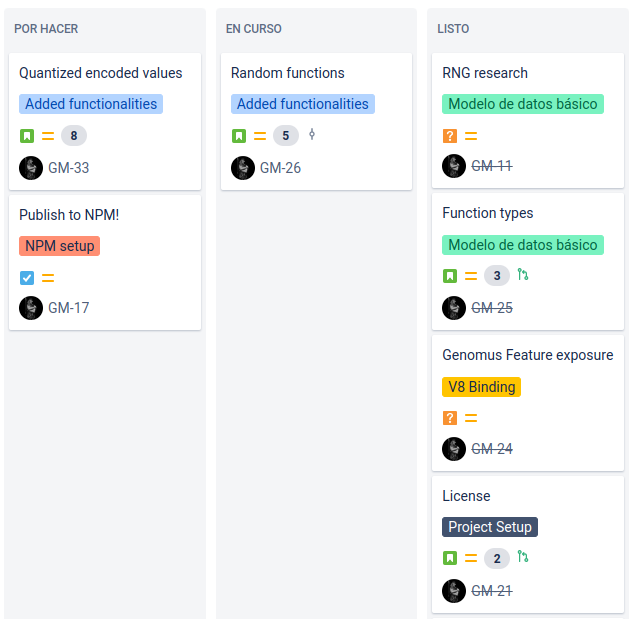
\includegraphics[width=\textwidth]{imagenes/kanban_04_07.png}
    \caption{Tablero KanBan del proyecto.} En su estado durante el último sprint, a fecha del 4 de julio de 2022.
    \label{fig:kanban_board}
\end{figure}

\subsubsection{Hitos e historias de usuario}

Las funcionalidades del MVP se han dividido en los siguientes hitos: 

\begin{itemize}
    \item \textit{Configuración del proyecto}. Hito en el que se han implementado las diferentes funcionalidades de despliegue del código y de control de versiones. Este hito ha incluido la configuración de los repositorios de git, la configuración del entorno de desarrollo y la creación de la integración circular.

    \item \textit{Modelo básico de datos}. Hito en el que se han implementado las funcionalidades más básicas para declarar genotipos y fenotipos, y realizar evaluaciones de genotipos.
    
    \item \textit{Funcionalidades añadidas}. Hito en el que se han incluidos las funcionalidades construidas sobre el modelo de datos. En este hito se incluyen el resto de transformaciones de datos, así como la representación de los datos como vectores numéricos normalizados.
        
    \item \textit{Enlace con V8}. Hito que ha incluido la investigación e implementación del enlace dinámico de nuestra librería compilada con el runtime de \verb|javascript|, que en este caso es el motor V8 al estar haciendo usode NodeJS\footnote{Más información en este artículo divulgativo de NodeJS sobre el motor V8: \url{https://nodejs.dev/learn/the-v8-javascript-engine}}.
    
    \item \textit{Publicación en NPM}. Hito que ha incluido la publicación del paquete \verb|genomus-core-js| en NPM.
\end{itemize}

Cada hito ha sido a su vez dividido en historias de usuario identificada de manera única por un código de historia. Al estar trabajando sobre el proyecto GenoMus, los códigos de historia siguen todos el formato \textit{GM-xxx}. En \ref{fig:roadmap} se puede ver como ha avanzado el progreso de los diferentes hitos, desglosado en historias de usuario individuales.

\begin{figure}
    \centering
    \centerline{
    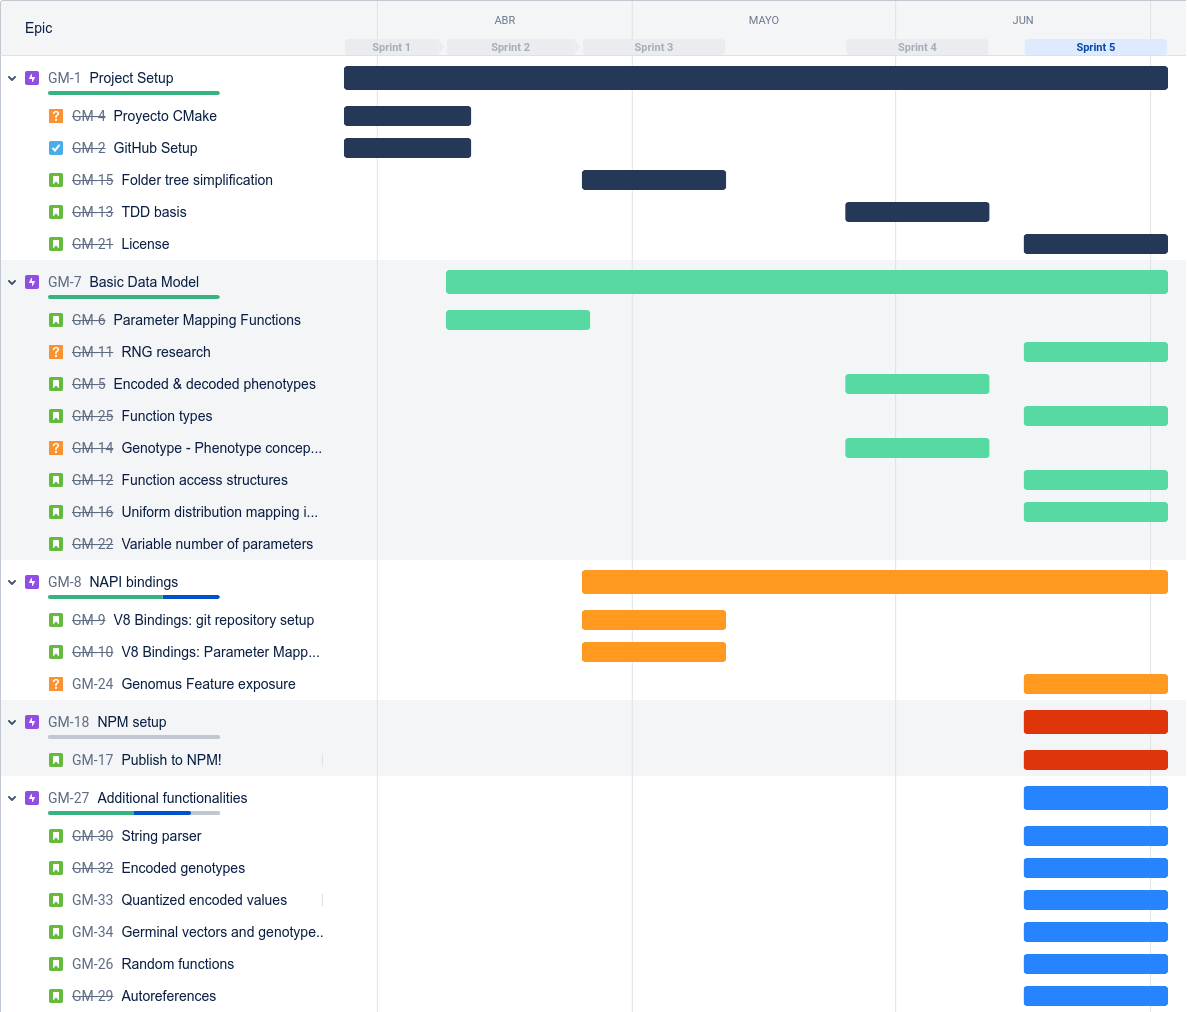
\includegraphics[width=0.8\paperwidth]{imagenes/road_map_03_07.png}
    }
    \caption{Hoja de ruta en proceso durante el sprint final del proyecto.}
    \label{fig:roadmap}
\end{figure}


\subsection{Protocolos de seguimiento del código}

Como se ha mencionado previamente, el proceso de desarrollo hace uso de un control de versiones con \verb|git| sobre repositorios alojados en Github y con una estructura de desarrollo que sigue un flujo de trabajo ampliamente inspirado en Gitflow. Se establecen los siguientes protocolos:

\subsubsection{Sobre ramas}

Las ramas utilizadas en el proyecto se clasifican en la rama principal \textit{master}, la rama de desarrollo \textit{develop} y las ramas de funcionalidad. Estas últimas están asociadas a una historia de usuario, cuyo código identificativo conforma el comienzo del nombre de la rama.

\subsubsection{Sobre mezclas}

La rama de desarrollo ramifica desde la rama principal, mientras que las ramas de funcionalidad ramifican desde la rama de desarrollo. Al finalizar una funcionalidad, la rama correspondiente se incorpora a la rama de desarrollo. Para realizar una \textit{release}, la rama de desarrollo se incorpora a la rama principal.
    
\subsubsection{Sobre peticiones de incorporación}

Las mezclas entre ramas estarán reflejadas en \textit{pull requests}, las cuales deberán tener un título descriptivo de las funcionalidades a incorporar y, opcionalmente, una descripción de estas. El único tipo de mezcla permitido en el proyecto es el \textit{squash and merge}\footnote{Refiriéndose a la funcionalidad de Github construida sobre el comando \textit{git merge --squash} consultable en la documentación oficial. \url{https://git-scm.com/docs/git-merge}}. Esto tiene el objetivo de mantener la limpieza de los \textit{logs}\footnote{Refiriéndose a los logs de git accesibles por el comando \textit{git log}. Más información en la documentación oficial de git. \url{https://www.git-scm.com/docs/git-log}} de las ramas de desarrollo y principal. Así, la rama de desarrollo solo registra un único \textit{commit} por historia de usuario, y la rama principal solo registra un commit por \textit{release}.
    
\subsubsection{Sobre tests automáticos}

La creación de una \textit{pull request} o el añadido de \textit{commits} a una rama observada por una \textit{pull request} debe disparar el lanzamiento de tests automáticos que comprueben la integridad de las funcionalidades previas a la rama. Idealmente se debe prohibir la incorporación de una rama con tests fallidos, pero esto es una funcionalidad que Github\footnote{Refiriéndose a la funcionalidad de \textit{reglas de protección de ramas} de Github. Consultable en la documentación oficial. \url{https://docs.github.com/en/repositories/configuring-branches-and-merges-in-your-repository/defining-the-mergeability-of-pull-requests/about-protected-branches}} no ofrece con su plan gratuíto, por lo que no se ha implementado.
    
\subsubsection{Sobre versionado semántico}

La publicación de una \textit{release} en la rama principal debe estar acompañada del etiquetado\footnote{Refiriéndose al etiquetado nativo de git, accesible a través del comando \textit{git tag} consultable en la documentación oficial. \url{https://git-scm.com/docs/git-tag}} de la rama principal con la versión del software a publicar.